\documentclass[11pt]{article}
\usepackage[textwidth=18.0cm, textheight=23.0cm, top=2.0cm]{geometry}
\usepackage{pst-all}
\usepackage{amssymb}
\usepackage{tikz}
\usepackage{underscore}\begin{document}
\pagestyle{empty}


ClassName: \underline{\textbf{Class_05.2bp-7}}
\par
BinSize: \underline{\textbf{100 × 100}}
\par
ReduceSize: \underline{\textbf{100 × 100}}
\par
TypeNum: \underline{\textbf{20}}
\par
Num: \underline{\textbf{20}}
\par
OutS: \underline{\textbf{50000}}
\par
InS: \underline{\textbf{40465}}
\par
Rate: \underline{\textbf{0.809}}
\par
UB: \underline{\textbf{5}}
\par
LB0: \underline{\textbf{5}}
\par
LB: \underline{\textbf{5}}
\par
LBWithCut: \underline{\textbf{5}}
\par
NodeCut: \underline{\textbf{0}}
\par
ExtendedNodeCnt: \underline{\textbf{1}}
\par
GenNodeCnt: \underline{\textbf{1}}
\par
PrimalNode: \underline{\textbf{0}}
\par
ColumnCount: \underline{\textbf{5}}
\par
TotalCutCount: \underline{\textbf{0}}
\par
RootCutCount: \underline{\textbf{0}}
\par
LPSolverCnt: \underline{\textbf{1}}
\par
PricingSolverCnt: \underline{\textbf{0}}
\par
BranchAndBoundNum: \underline{\textbf{1}}
\par
isOpt: \underline{\textbf{true}}
\par
TimeOnPrimal: \underline{\textbf{0.000 s}}
\par
TimeOnPricing: \underline{\textbf{0.000 s}}
\par
TimeOnRmp: \underline{\textbf{0.078 s}}
\par
TotalTime: \underline{\textbf{0.140 s}}
\par
\newpage


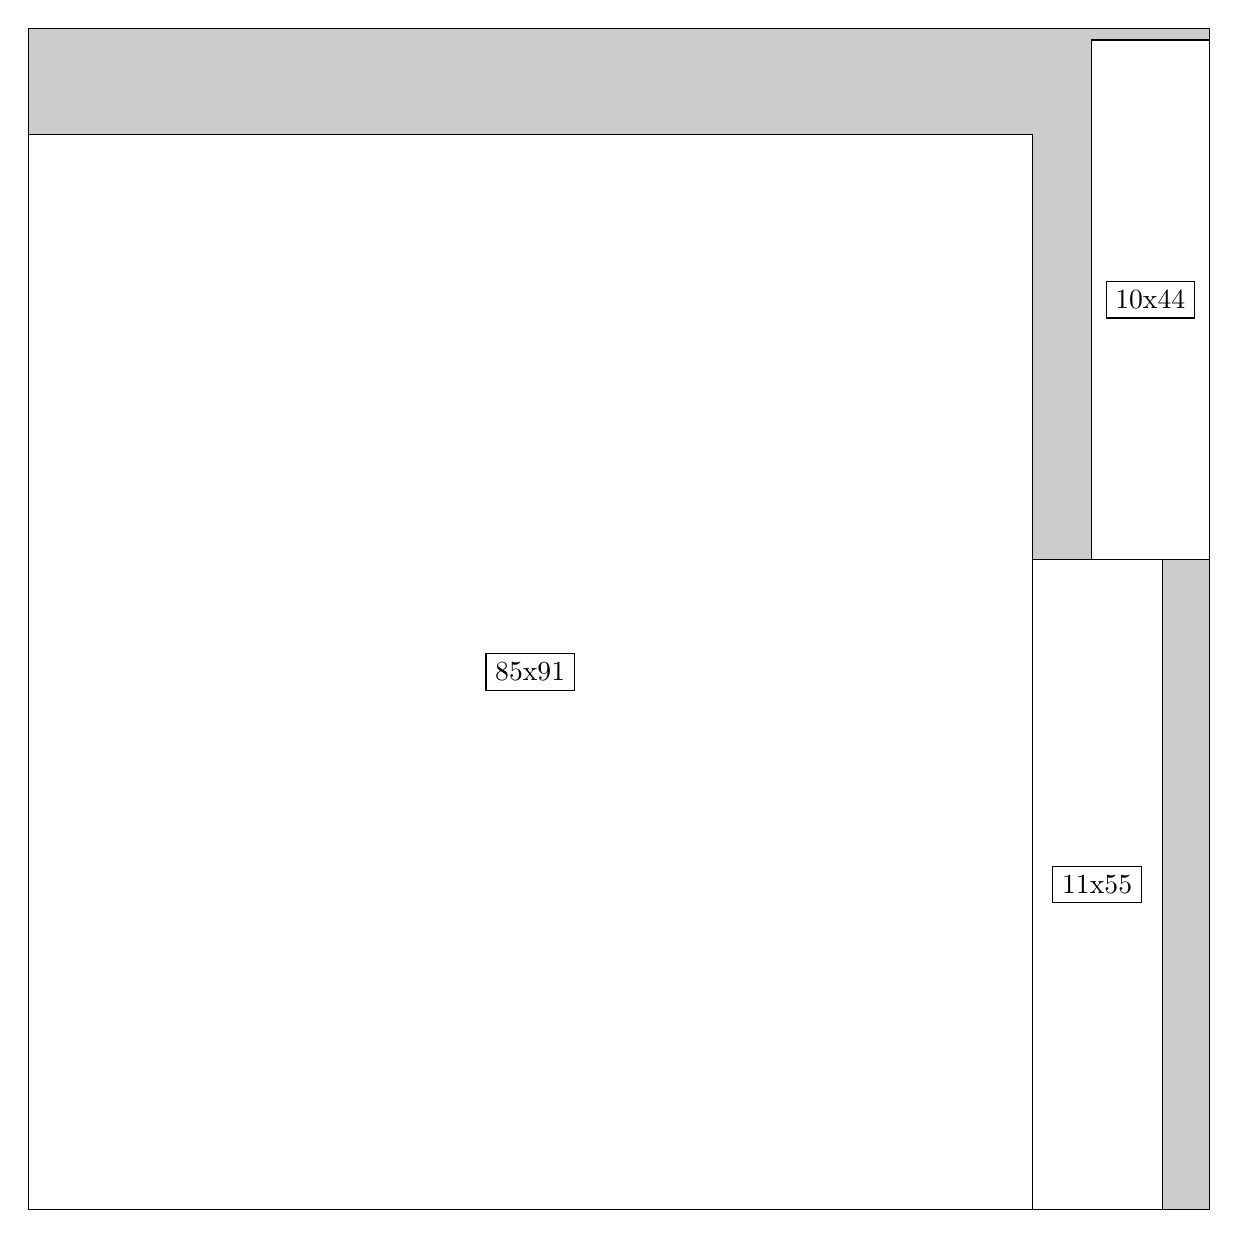
\begin{tikzpicture}[shorten >=1pt,scale=1.0,every node/.style={scale=1.0},->]
\tikzstyle{vertex}=[circle,fill=black!25,minimum size=14pt,inner sep=0pt]
\filldraw[fill=gray!40!white, draw=black] (0,0) rectangle (15.0,15.0);
\foreach \name/\x/\y/\w/\h in {85x91/0.0/0.0/12.75/13.65,11x55/12.75/0.0/1.65/8.25,10x44/13.5/8.25/1.5/6.6}
\filldraw[fill=white!40!white, draw=black] (\x,\y) rectangle node[draw] (\name) {\name} ++(\w,\h);
\end{tikzpicture}


w =85 , h =91 , x =0 , y =0 , v =7735
\par
w =11 , h =55 , x =85 , y =0 , v =605
\par
w =10 , h =44 , x =90 , y =55 , v =440
\par
\newpage


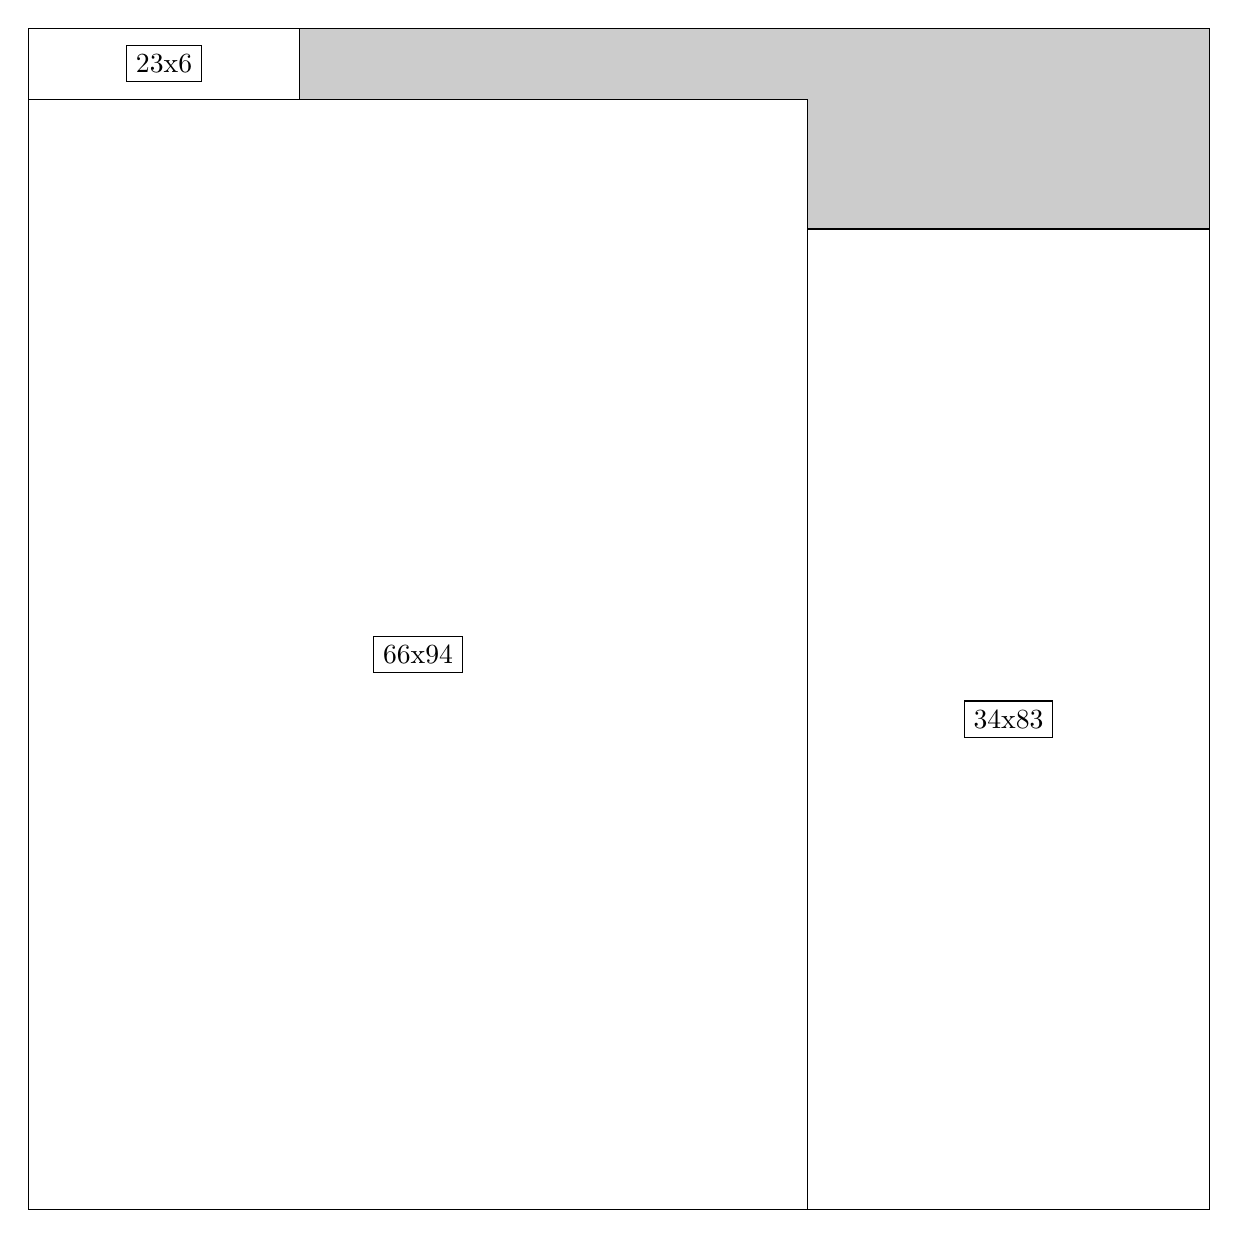
\begin{tikzpicture}[shorten >=1pt,scale=1.0,every node/.style={scale=1.0},->]
\tikzstyle{vertex}=[circle,fill=black!25,minimum size=14pt,inner sep=0pt]
\filldraw[fill=gray!40!white, draw=black] (0,0) rectangle (15.0,15.0);
\foreach \name/\x/\y/\w/\h in {66x94/0.0/0.0/9.9/14.1,34x83/9.9/0.0/5.1/12.45,23x6/0.0/14.1/3.4499999999999997/0.8999999999999999}
\filldraw[fill=white!40!white, draw=black] (\x,\y) rectangle node[draw] (\name) {\name} ++(\w,\h);
\end{tikzpicture}


w =66 , h =94 , x =0 , y =0 , v =6204
\par
w =34 , h =83 , x =66 , y =0 , v =2822
\par
w =23 , h =6 , x =0 , y =94 , v =138
\par
\newpage


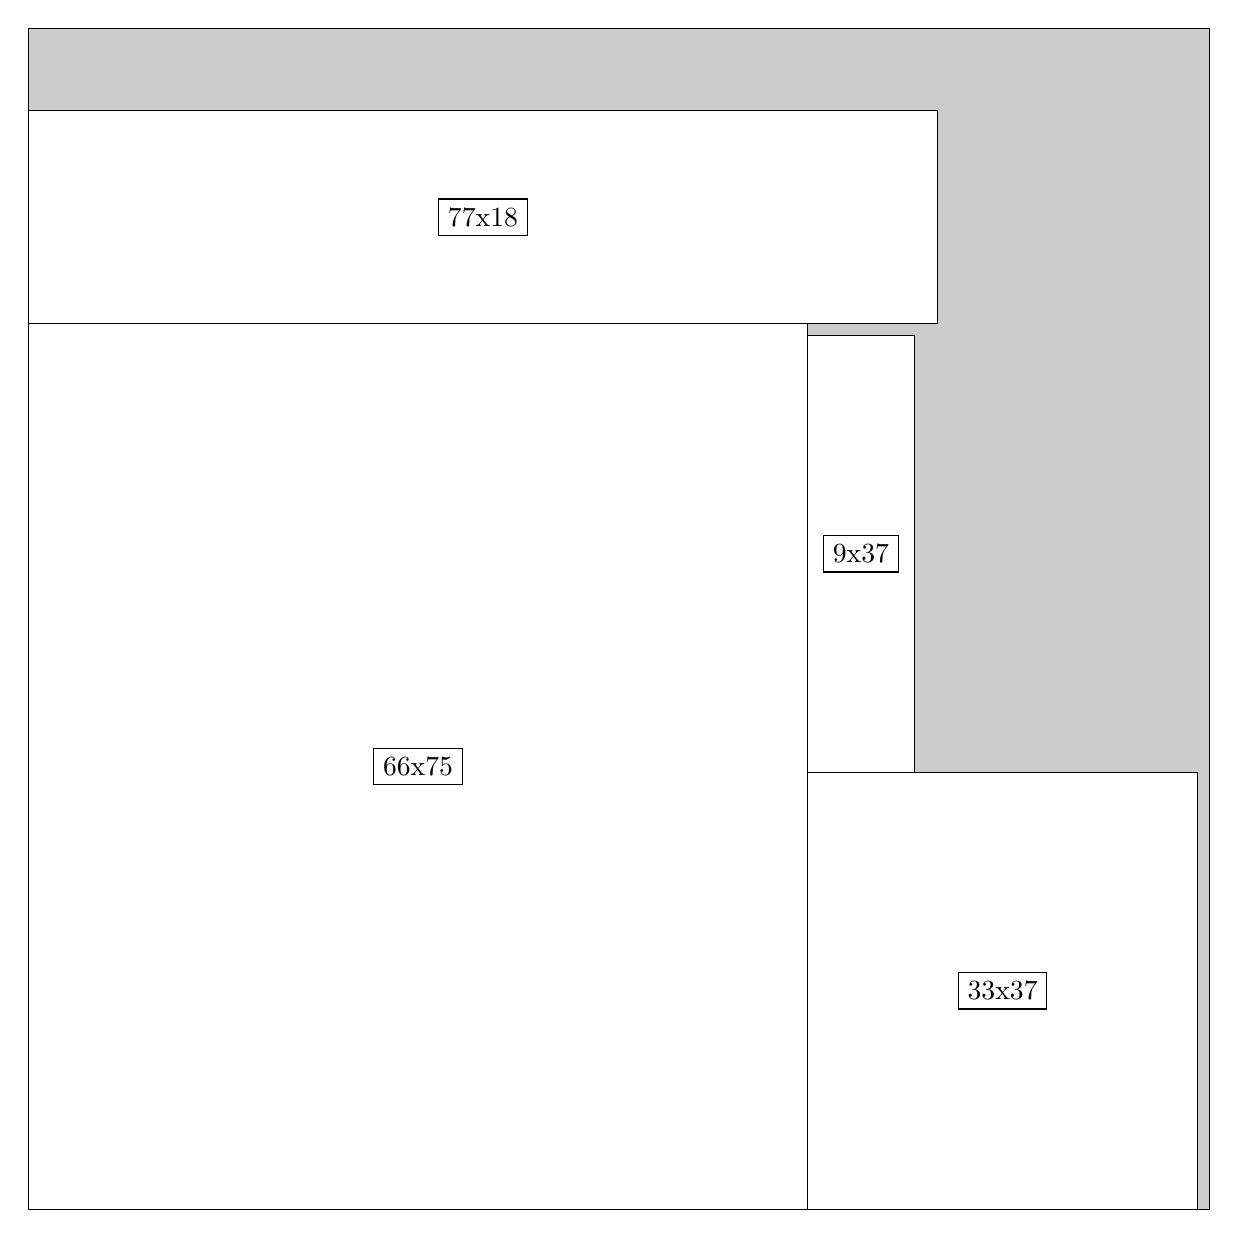
\begin{tikzpicture}[shorten >=1pt,scale=1.0,every node/.style={scale=1.0},->]
\tikzstyle{vertex}=[circle,fill=black!25,minimum size=14pt,inner sep=0pt]
\filldraw[fill=gray!40!white, draw=black] (0,0) rectangle (15.0,15.0);
\foreach \name/\x/\y/\w/\h in {66x75/0.0/0.0/9.9/11.25,77x18/0.0/11.25/11.549999999999999/2.6999999999999997,33x37/9.9/0.0/4.95/5.55,9x37/9.9/5.55/1.3499999999999999/5.55}
\filldraw[fill=white!40!white, draw=black] (\x,\y) rectangle node[draw] (\name) {\name} ++(\w,\h);
\end{tikzpicture}


w =66 , h =75 , x =0 , y =0 , v =4950
\par
w =77 , h =18 , x =0 , y =75 , v =1386
\par
w =33 , h =37 , x =66 , y =0 , v =1221
\par
w =9 , h =37 , x =66 , y =37 , v =333
\par
\newpage


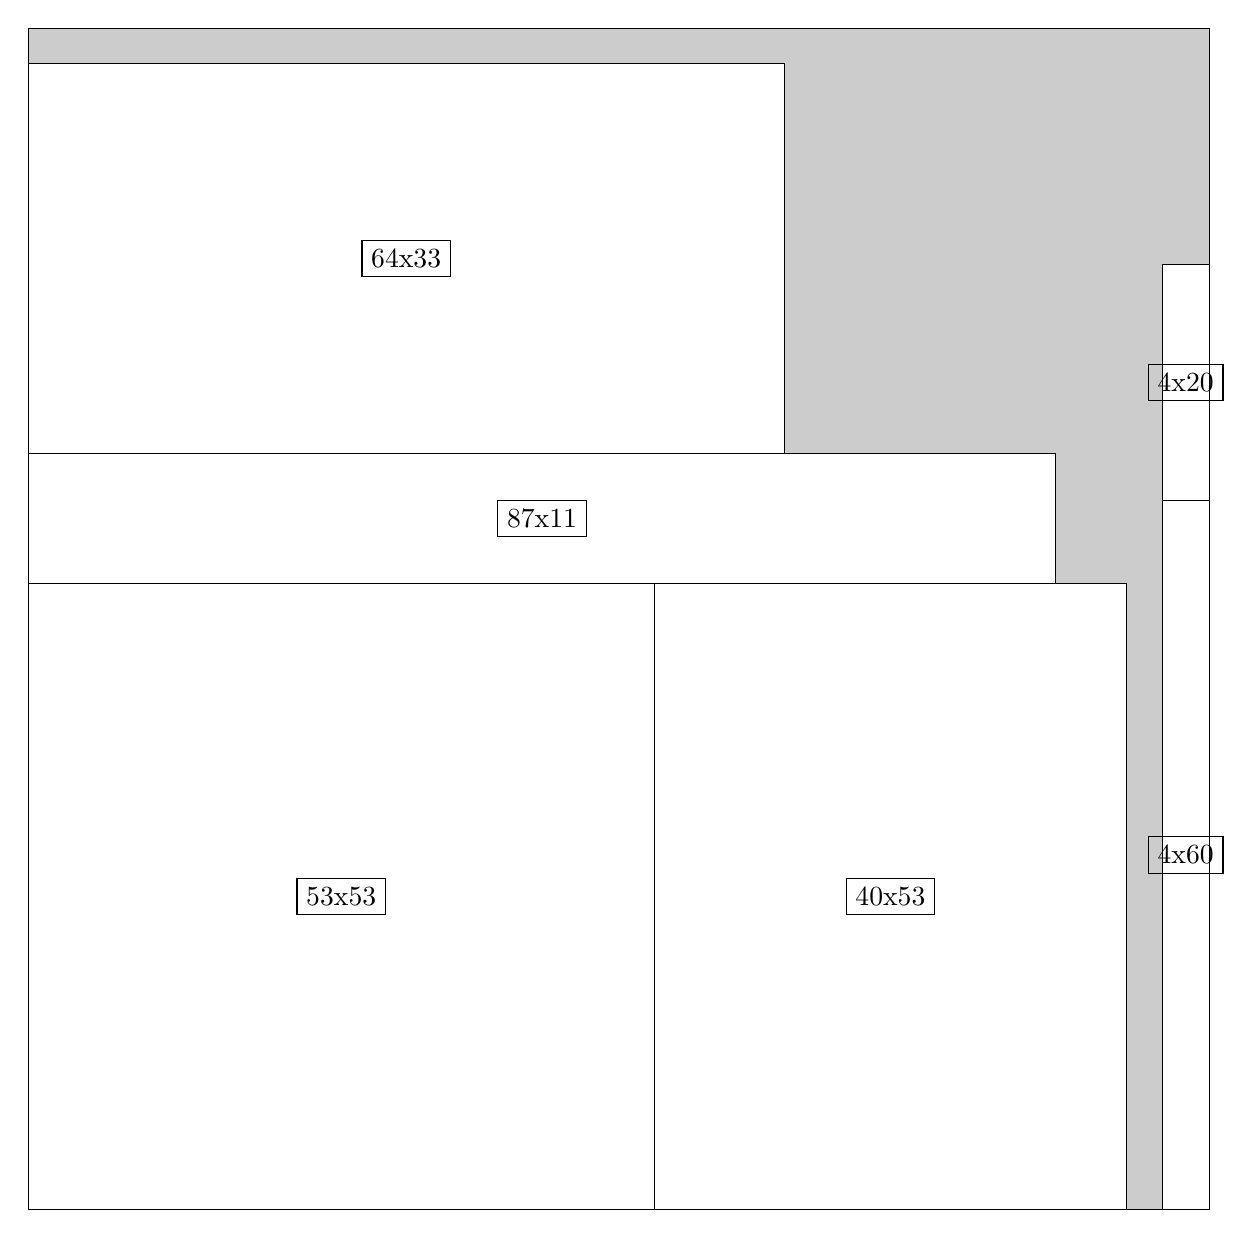
\begin{tikzpicture}[shorten >=1pt,scale=1.0,every node/.style={scale=1.0},->]
\tikzstyle{vertex}=[circle,fill=black!25,minimum size=14pt,inner sep=0pt]
\filldraw[fill=gray!40!white, draw=black] (0,0) rectangle (15.0,15.0);
\foreach \name/\x/\y/\w/\h in {53x53/0.0/0.0/7.949999999999999/7.949999999999999,40x53/7.949999999999999/0.0/6.0/7.949999999999999,64x33/0.0/9.6/9.6/4.95,87x11/0.0/7.949999999999999/13.049999999999999/1.65,4x60/14.399999999999999/0.0/0.6/9.0,4x20/14.399999999999999/9.0/0.6/3.0}
\filldraw[fill=white!40!white, draw=black] (\x,\y) rectangle node[draw] (\name) {\name} ++(\w,\h);
\end{tikzpicture}


w =53 , h =53 , x =0 , y =0 , v =2809
\par
w =40 , h =53 , x =53 , y =0 , v =2120
\par
w =64 , h =33 , x =0 , y =64 , v =2112
\par
w =87 , h =11 , x =0 , y =53 , v =957
\par
w =4 , h =60 , x =96 , y =0 , v =240
\par
w =4 , h =20 , x =96 , y =60 , v =80
\par
\newpage


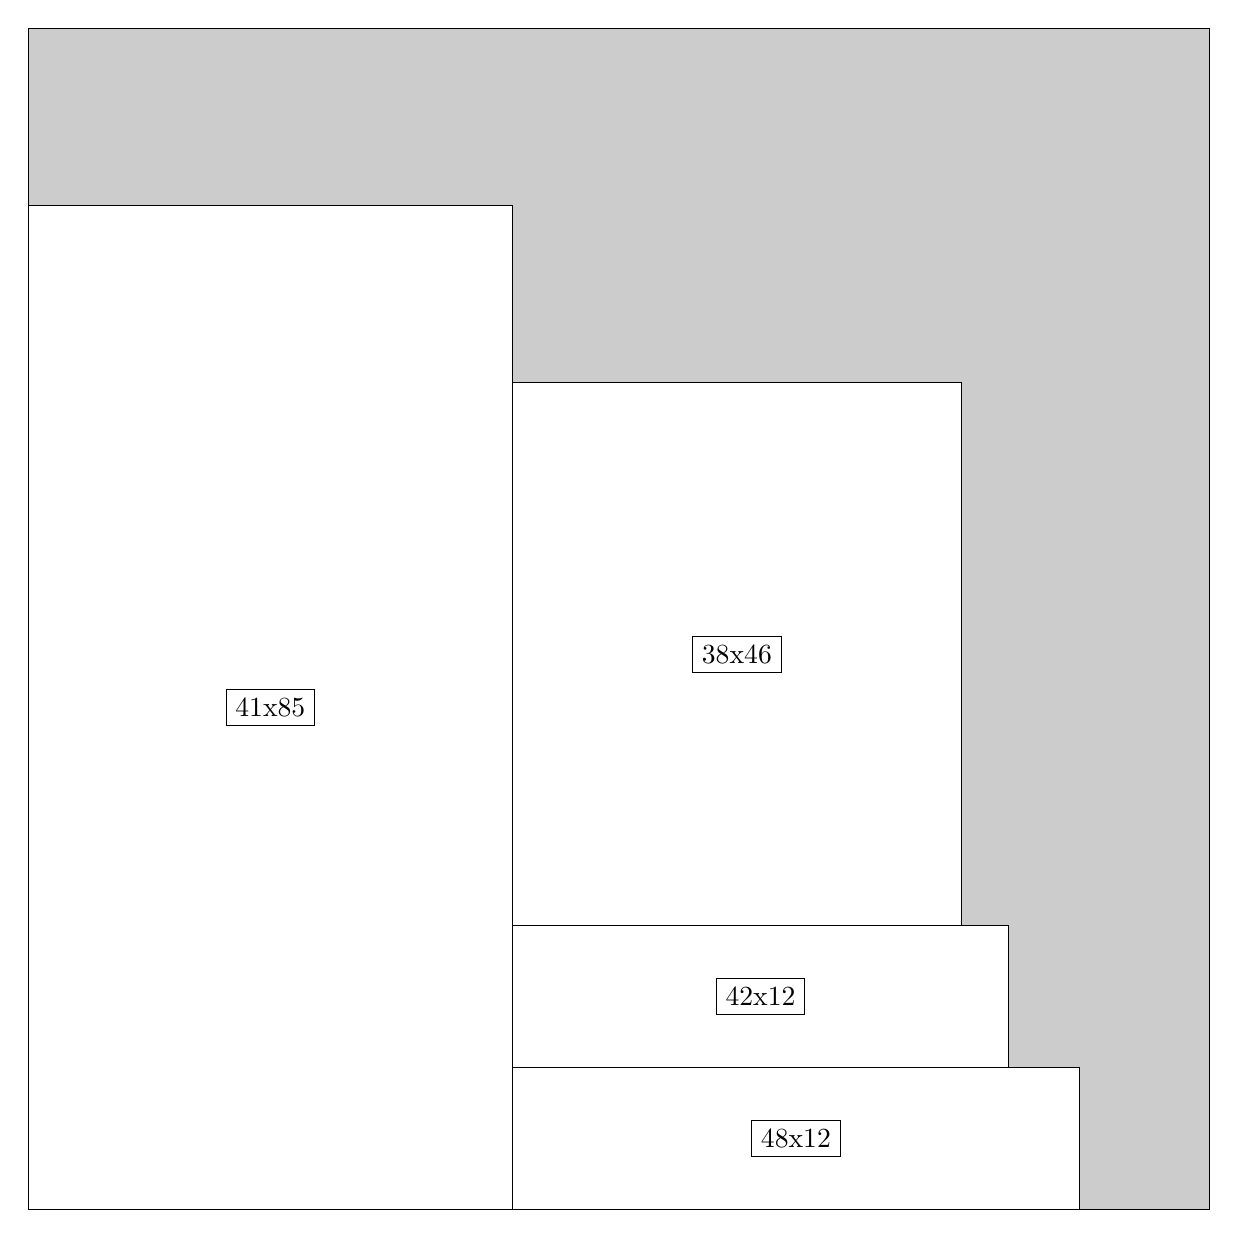
\begin{tikzpicture}[shorten >=1pt,scale=1.0,every node/.style={scale=1.0},->]
\tikzstyle{vertex}=[circle,fill=black!25,minimum size=14pt,inner sep=0pt]
\filldraw[fill=gray!40!white, draw=black] (0,0) rectangle (15.0,15.0);
\foreach \name/\x/\y/\w/\h in {41x85/0.0/0.0/6.1499999999999995/12.75,38x46/6.1499999999999995/3.5999999999999996/5.7/6.8999999999999995,48x12/6.1499999999999995/0.0/7.199999999999999/1.7999999999999998,42x12/6.1499999999999995/1.7999999999999998/6.3/1.7999999999999998}
\filldraw[fill=white!40!white, draw=black] (\x,\y) rectangle node[draw] (\name) {\name} ++(\w,\h);
\end{tikzpicture}


w =41 , h =85 , x =0 , y =0 , v =3485
\par
w =38 , h =46 , x =41 , y =24 , v =1748
\par
w =48 , h =12 , x =41 , y =0 , v =576
\par
w =42 , h =12 , x =41 , y =12 , v =504
\par
\newpage


\end{document}